\documentclass{beamer}
\usetheme{Warsaw}
\usecolortheme{seahorse}

\usepackage{graphicx}
\usepackage{listings} 
\usepackage{placeins}
\usepackage{amsmath,amsfonts,mathrsfs}
\usepackage{tikz}
\usepackage{url}
\usepackage{amssymb}
\usepackage{circuitikz}
\usepackage{xcolor}
\usepackage{gensymb}
\usepackage{array}
\usepackage{tabularx}

\usepackage{sansmathaccent}
\pdfmapfile{+sansmathaccent.map}

\usetikzlibrary{angles}

\title[Potentiometric Roll Angle Displacement Measurement] 
{Potentiometric-based Smart Transducer for Roll Angle Estimation}
\subtitle{ELEN4006 Project Presentation}
\author % (optional, for multiple authors)
{M.~van~Rooyen \and J.~Ping}
\institute[Wits] % (optional)
{
  School of Electrical and Information Engineering, \\
  University of the Witwatersrand
}
\date{26 April 2018}
\subject{Measurements}

\setbeamertemplate{sidebar right}{}
\setbeamertemplate{footline}{%
	\hfill\usebeamertemplate***{navigation symbols}
	\hspace{0.5cm}\insertframenumber{}/\inserttotalframenumber}

\begin{document}
	
\frame{\titlepage}

\begin{frame}
	\frametitle{Table of Contents}
	\tableofcontents[ 
	currentsection, 
	currentsubsection, 
	sectionstyle=show, 
	subsectionstyle=show, 
	] 
\end{frame}

\section{System Overview}
\begin{frame}
\frametitle{Problem Statement}

\begin{itemize}
	\item Active safety control system prevents unwanted driver conditions
	\item Angular displacement measured at the wheel base
	\item Control system must have accurate readings of the roll angle.
	\item A number of environmental conditions affect this:
	\setlength{\itemindent}{.3in}
	\item Road vibrations 
	\item Tyre pressure 
	\item Motor vibrations.
\end{itemize}
\end{frame}

\begin{frame}
\frametitle{Block Diagram}
\tikzstyle{block} = [rectangle, draw, text width=6.5em, text centered, color=black, minimum height=4em]   
\begin{tikzpicture}[->,transform canvas={scale=.75}, >=triangle 45,auto]
\draw
node at (0em,3em) [coordinate] (start) {}
node at (7em,3em) [block, fill=blue!40] (pot) {Potentiometer}
node at (19em,3em) [block, fill=purple!40] (wb) {Wheatstone Bridge}
node at (31em,3em) [block, fill=purple!40] (ia) {Instrumentation Amplifier}
node at (34em,-5em) [block, fill=purple!40] (aaf) {Anti-aliasing Filter}
node at (25em,-5em) [block, fill=red!40] (adc) {ADC}
node at (16em,-5em) [block, fill=red!40] (uc) {MCU}
node at (7em,-5em) [block, fill=green!40] (lcd) {Control System}
node at (0em,-5em) [coordinate] (end) {}

node at (1em, -12em) [block, fill=blue!40, minimum height = 1em, text width = 0.5em, label={[label distance=0.5em]0:Sensing}] (k1) {}
node at (7.5em, -12em) [block, fill=purple!40, minimum height = 1em, text width = 0.5em, label={[label distance=0.5em]0:Conditioning}] (k1) {}
node at (16em, -12em) [block, fill=red!40, minimum height = 1em, text width = 0.5em, label={[label distance=0.5em]0:Processing}] (k1) {}
node at (24em, -12em) [block, fill=green!40, minimum height = 1em, text width = 0.5em, label={[label distance=0.5em]0:Data Presentation}] (k1) {}
;

\path
(start) edge[] node[above] {$\theta$} (pot)
(pot) edge[] node[above] {\ohm} (wb)
(wb) edge[] node[above] {V} (ia)
(ia) edge[bend left] node[right] {V} (aaf)
(aaf) edge[] node[above] {V} (adc)
(adc) edge[] node[above] {V} (uc)
(uc) edge[] node[above] {V} (lcd)
(lcd) edge[] node[above] {$\theta$} (end)
;
\end{tikzpicture}

\end{frame}

\section{Sensing}

\begin{frame}
\frametitle{Angular Potentiometer}
\framesubtitle{Diagram}

\begin{columns}[T]
	\begin{column}[T]{0.4\textwidth}
		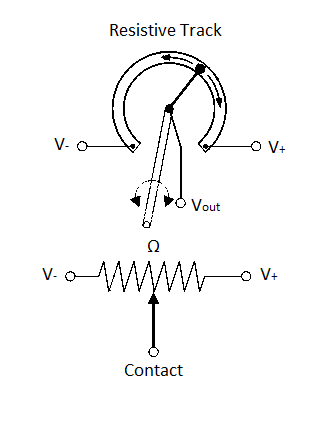
\includegraphics[width=\textwidth]{Pot2.png}
	\end{column}
	\begin{column}[T]{0.6\textwidth}
		\vspace{0.5cm}
		\begin{tabular}{|p{0.3\textwidth}| p{0.35\textwidth}|}
			\hline
			\textbf{Element} & \textbf{Material} \\ \hline
			Resistor & Conductive Plastic Paste\\ \hline
			Terminals & Thick film conductor \\ \hline
			Contact & Multiple-fingered equidistant wiper\\ \hline
			Actuator & Rotary Shaft \\
			\hline
		\end{tabular}
	\end{column}
	
\end{columns}

\end{frame}

\begin{frame}
\frametitle{Angular Potentiometer}
\framesubtitle{Circuit Diagram}

\begin{columns}[T]
	\begin{column}[T]{0.5\textwidth}
		\centering
		\begin{tabular}{|p{0.2\textwidth}| p{0.15\textwidth}| p{0.15\textwidth}|}
			\hline
			Roll Angle ($\degree$) & $\mathrm{R_{pot}}$ $~($k$\Omega)$ & $\mathrm{V_{out}}$ $~(\mathrm{V})$ \\ \hline
			-15 & 1 & 0 \\
			15 & 12 & 5 \\ \hline
		\end{tabular}
	
	\vspace{0.5cm}
	
		\begin{circuitikz}[american voltages, transform shape, scale=0.6]
		% Voltage source
		\draw (0,0) to [-*] (3,0)
		to [american potentiometer,n=mypot, o-o] (3,-4)
		(0,-4) to [short,-] (6,-4)
		(mypot.wiper) to[short] (6,-2)
		to [short] (6,0) to [short] (3,0);
		\draw (6,-2.2) node[open] {+}
		(6,-3.8) node[open] {-}
		(6,-3) node[open] {$\mathrm{V_{out}}$};
		\draw (4.1,-2.3) node[open] {$\uparrow$}
		(4.1,-3.7) node[open] {$\downarrow$}
		(4.1,-3) node[open] {$\beta~\mathrm{R_{pot}}$};
		\draw (4.1,-0.3) node[open] {$\uparrow$}
		(4.1,-1.7) node[open] {$\downarrow$}
		(4.1,-1) node[open] {$(1-\beta)~\mathrm{R_{pot}}$}
		(2,-2) node[open] {$\mathrm{R_{pot}}$};
		\draw (0,-1) node[open] {+}
		(0,-3) node[open] {-}
		(0,-2) node[open] {$\mathrm{V_{in}}$};
	\end{circuitikz}
	\end{column}
	\begin{column}[T]{0.5\textwidth}
		\textbf{Resistive Element}
		\begin{itemize}
			\item Carbon black inert filler
			\item Strong with long lifespan
			\item Very high resolution
			\item Positive Temperature Coefficient $\pm 100~\mathrm{ppm/\degree C}$
			\item non-linearity of $\sim 0.4~\%$
		\end{itemize}
	\end{column}
\end{columns}
\end{frame}

\section{Signal Conditioning}
\begin{frame}
\frametitle{Wheatstone Bridge}
\framesubtitle{Signal Conditioning Element}

\def\x{6}
\def\y{6}
% Size of the bridge
\def\dx{3}
\def\dy{3}

\begin{columns}[T]
	\begin{column}[T]{0.55\textwidth}
		\begin{circuitikz}[american voltages, transform shape, scale=0.6]
			% Voltage source
			\draw (0,0) to [V, l_=$\mathrm{V_s:~51V}$]
			(0, \y) to [R, l_=$\mathrm{R_s:}~50~\Omega$, -*] (\x, \y)
			% Left half bridge
			to [R, l_=$\mathrm{R(x)}$, *-] (\x-\dx,\y-\dy) % Top left resistor
			to [R, l_=100~$\mathrm{k}\Omega$, -*] (\x,\y-2*\dy);  % Bottom left resistor
			% Right half bridge
			\draw (\x,\y)
			to [R, l_=100~$\Omega$] (\x+\dx, \y-\dy) % Top right resistor
			to [R, l_=10~$\mathrm{k}\Omega$, -*] (\x,\y-2*\dy)  % Bottom left resistor
			% Draw connection to (-) terminal of voltage source
			to (\x, 0) to (0,0);
			
			% Draw Vout
			\draw (\x-\dx,\y-\dy) to [short, -*] (\x-\dx+1,\y-\dy)
			(\x+3,\y-\dy) to [short, -*] (\x+2,\y-\dy);
			\draw (\x-\dx+1.5,\y-\dy) node[open] {+};
			\draw (\x+1.5,\y-\dy) node[open] {-};
			\draw (\x,\y-\dy) node[open] {$\mathrm{V_{out}}$};
		\end{circuitikz}
	\end{column}
	\begin{column}[T]{0.45\textwidth}
		\begin{itemize}
			\item $i_{\mathrm{max}}$ at $\mathrm{V_{out}}$ = $1.3~\mathrm{mA}$
			\item $\mathrm{P_{max}} = 16.9~\mathrm{mW}$
			\item Resistor tolerances = $0.5~\%$
			\item Bandwidth $\approxeq 1~\mathrm{GHz}$
			\item Power Supply (PSU): Output Voltage 51~V $\pm 1~\%$, output resistance of $50~\Omega$
	\end{itemize}
	\end{column}
\end{columns}

\end{frame}

\begin{frame}
\frametitle{Instrumentation Amplifier}
\framesubtitle{Signal Conditioning Element}

\textbf{Texas Instruments INA188}

\begin{itemize}
	\item 3 Op-amp IC
	\item G $ = 1 $
	\item BW $ = 600~\mathrm{kHz} $
	\item $ \mathrm{E_G} = \pm 0.025~\% $ (worst case)
	\item Input Bias Current: $2.5~\mathrm{pA}$
	\item Input Offset Current: $2.5~\mathrm{pA}$
	\item Input Impedance: $100~\mathrm{G\Omega}$
	\item Operating Temperature Range: $-55~^\circ \mathrm{C}$ - $150~^\circ \mathrm{C}$
	\item Supply Voltage Range: $4~\mathrm{V}$ - $36~\mathrm{V}$
\end{itemize}
\end{frame}

\begin{frame}
\frametitle{Anti-aliasing Filter}
\framesubtitle{Signal Conditioning Element}

\begin{columns}[T] % contents are top vertically aligned
	\begin{column}[T]{0.5\textwidth} % each column can also be its own environment
		\centering
		2nd Order Butterworth LPF
		\vspace{0.5cm}
		\begin{circuitikz}[transform shape,scale=0.75]\draw
			(5,-0.5) node[op amp, yscale=-1](opamp){}
			(-1,0) node[left] {} to [R, l=$R_1$, o-] (1,0)
			to [R, l=$R_2$, -] ($(opamp.+)+(-1,0)$)
			to [C, l_=$C_2$, -] ($(opamp.+)+(-1,-2)$) node[ground] {}	
			($(opamp.+)+(-1,0)$) to [-] (opamp.+)	
			(opamp.out) to [-] ($(opamp.out)+(0,1.5)$) 
			to [C, l_=$C_1$, -] ($(opamp.+)+(-1,1)$)
			to [-] ($(opamp.+)+(-1,0)$)
			(opamp.-) to [-] ($(opamp.-)+(0,-1)$)
			to [-] ($(opamp.out)+(0,-1.5)$)
			to [-] (opamp.out)
			to [-] ($(opamp.out)+(0.5,0)$)
			;	 
		\end{circuitikz}
	\end{column}
	\begin{column}[T]{0.5\textwidth} % alternative top-align that's better for graphics
		\centering
		\begin{tabular}{|l|l|}
			\hline
			\textbf{Element} & \textbf{Value} \\ \hline
			$ \mathrm{R_1} $ & $ \mathrm{10 k \Omega} $ \\
			$ \mathrm{R_2} $ & $ \mathrm{10 k \Omega} $ \\
			$ \mathrm{C_1} $ & $ \mathrm{3.60 n F} $ \\
			$ \mathrm{C_2} $ & $ \mathrm{7.21 n F} $ \\ \hline
		\end{tabular}
		\begin{displaymath}    
		Q = \frac{\sqrt{\mathrm{R_1 R_2 C_1 C_2}}}{C_2 (R_1 + R_2)} \approxeq 0.707
		\end{displaymath}
		\begin{displaymath}    
		f_c = \frac{1}{2 \pi \sqrt{R_1 R_2 C_1 C_2}} = 3.12~kHz
		\end{displaymath}
	\end{column}
\end{columns}	 

\end{frame}

\begin{frame}
\frametitle{Anti-aliasing Filter}
\framesubtitle{Signal Conditioning Element}
\centering
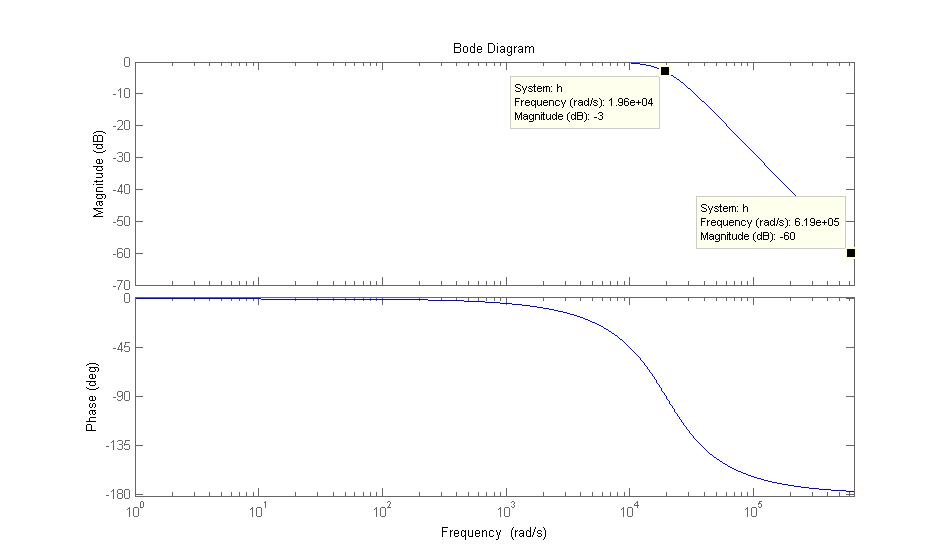
\includegraphics[height=0.73\textheight]{filterBode} 
\begin{displaymath}    
f_c \sim 19.6~\mathrm{kRad.s^{-1}} = 3.12~\mathrm{kHz}, \quad f_{0.1\%} \sim 619~\mathrm{kRad.s^{-1}} = 98.5~\mathrm{kHz}
\end{displaymath}

\end{frame}

\begin{frame}
\frametitle{Anti-aliasing Filter}
\framesubtitle{Signal Conditioning Element}

\textbf{Texas Instruments - LMC6022 Operational Amplifier}
\begin{itemize}
	\item Input Bias Current: $200~\mathrm{pA}$
	\item Input Offset Current: $100~\mathrm{pA}$
	\item Input Impedance: $1~\mathrm{T\Omega}$
	\item Operating Temperature Range: $-40^\circ \mathrm{C}$ - $85^\circ \mathrm{C}$
	\item Supply Voltage Range: $4.5~\mathrm{V}$ - $15.5~\mathrm{V}$
	\item Resistor tolerances: $0.5~\%$ 
	\item Capacitor tolerances: $0.5~\%$
\end{itemize}

\begin{displaymath}    
H(s) = \frac{1}{1 + 14.4 \times 10^{-6}s + 25.96 \times 10^{-12}s^2}
\end{displaymath}

\end{frame}

\section{Signal Processing}
\begin{frame}
\frametitle{Analog to Digital Converter}
\framesubtitle{Signal Processing Element}

\begin{itemize}
	\item $f_{0.1\%} = 98.5~\mathrm{kHz}$
	\item $ \therefore $ sample at minimum $ \mathrm{f_s} = 200~\mathrm{kHz} $ to satisfy Nyquist sampling theorem
	\item $ \therefore 0.1 \% $ aliasing error
	\item 10 bit resolution
	\item $ \therefore \frac{1}{2^{10}}\times 100\% = \frac{1}{1024} \times 100 \% = 0.098 \% $ quantization error
\end{itemize}
\end{frame}
\begin{frame}
\frametitle{Microprocessor}
\framesubtitle{Signal Processing Element}

\textbf{Microchip - dsPIC30F2010}
\begin{itemize}
\item $7.37~\mathrm{MHz}$ internal oscillator
\item $6 \times 10$ bit, 1000 ksps ADC
\item 20 I/O pins
\item Operating Temperature Range: $-40^\circ \mathrm{C}$ - $125^\circ \mathrm{C}$
\item Operating Voltage Range: $2.5~\mathrm{V}$ - $5.5~\mathrm{V}$
\end{itemize}
\end{frame}

\section{Error Analysis}
\begin{frame}
\frametitle{Error Analysis}
\begin{tabular}{|l|l|}
	\hline
	\textbf{Source} & \textbf{Value $\%$} \\ \hline
	Conductive plastic non-linearity & 0.4~$\%$ \\
	Potentiometer contact resistance variation (CRV) & 0.075~$\%$ \\
	Wheatstone bridge non-linearity & 2.33~$\%$\\
	Instrumentation amplifier gain error & 0.025$\%$ \\
	Aliasing error & 0.1~$\%$ \\
	Resistor tolerance & 0.5~$\%$ \\
	Capacitor tolerance & 0.5~$\%$ \\
	Quantization error & 0.098~$\%$ \\ \hline
	\textbf{Total error} &  \textbf{4.028~$\%$} \\ \hline
\end{tabular}

\end{frame}

\begin{frame}
\frametitle{Bentley's Model}

\begin{flalign}
O &= KI + a + N(I) + K_MI_MI + K_II_I \\
O &= 0.1I + 2.1 + 33.6\times10^{-3} + 0.1\cdot0.26I + 0.2\times10^{-6} I_I \nonumber
\end{flalign}
\vspace{-0.5cm}
\begin{columns}[T]
	\begin{column}[T]{0.5\textwidth}
		\begin{itemize}
			\item O = Steady-state output $0\mathrm{V}~\mathrm{to}~5\mathrm{V}$
			\item K = sensitivity ($\mathrm{V/\degree}$)
			\item I = Input: $-15\degree~\mathrm{to}~15\degree$
			\item \textit{a} = Zero bias (V)
			\item $N(I)_{\mathrm{max}}$ = 33.6mV %0.6728\%
			\item $K_M$ = Change in sensitivity for modifying input
		\end{itemize}
	\end{column}
	\begin{column}[T]{0.5\textwidth}
		\begin{itemize}
			\item $I_M$ = $\pm1\%$ error in PSU output
			\item $K_I$ = Sensitivity change due to $I_I$ ($\mathrm{V/\degree C}$)
			\item $I_I$ = Difference between operating temperature and $25\degree\mathrm{C}$
		\end{itemize}
	\end{column}
	
\end{columns}
\end{frame}

\section{Conclusion}
\begin{frame}
\frametitle{Smart Transducer Requirements}
Core functionality:
\begin{itemize}
	\item Transduction
	\item Signal Conditioning
	\item Signal Processing
	\item Communication
	\item Memory
\end{itemize}
Added functionality:
\begin{itemize}
	\item Averaging of multiple devices
	\item Self calibration - differential between each wheel base
	\item Self diagnosing
\end{itemize}  

\end{frame}
\begin{frame}
\frametitle{Further Work}
\begin{itemize}
\item Digital Filtering
\item Costing
\item Finalise all components
\item Power Supply
\end{itemize}

\end{frame}

\begin{frame}
\frametitle{Conclusion}
Any questions?
\end{frame}
	
\end{document}